\documentclass[9pt]{article}

\usepackage{graphicx} % Required for inserting images
\usepackage{amsmath}
\usepackage{amsfonts}
\usepackage{ctex}
\usepackage{enumitem}
\usepackage{longtable}
\usepackage{makecell} % 换行

% 使用分栏宏包
\usepackage{multicol} 
\setlength{\columnseprule}{0.4pt} % 分割线

% 设置字体
\usepackage{unicode-math}
\setmainfont{Cambria}
\setmathfont{Cambria Math}

% 调整页面布局
\usepackage[a4paper, top=0.7cm, bottom=1cm, left=0.7cm, right=.7cm]{geometry}
\setlength{\footskip}{15pt}

% 设置页脚/页眉
\usepackage{fancyhdr}
\fancyfoot[C]{Copyright By Jingren Zhou | Page \thepage}
\fancyhead[]{}
\pagestyle{fancy}
% 去除线
\renewcommand{\headrulewidth}{0pt}
\renewcommand{\footrulewidth}{0pt}

% 设置 section/subsection 之间的行间距
\usepackage{titlesec}
\titlespacing*{\section}{0pt}{-2pt}{-2pt}
\titlespacing*{\subsection}{0pt}{-2pt}{-2pt}

% 调整标题上下间距
\usepackage{titling}
\setlength{\droptitle}{-2.4cm} % 负值表示向上移动

% 设置标题,作者,时间
\title{HCV Note}
\author{}
\date{}

% 正文
\begin{document}

\newcommand{\np}{{\tiny $^{^{^\ominus}}$}}

% 标题
\maketitle
\thispagestyle{fancy}
\vspace{-3.5cm}

% 字体大小
\fontsize{10pt}{11pt}\selectfont
\setlength{\parindent}{8pt}

\section{Basic Knowledge} % Basic Knowledge

\textbf{Useful Complex Number Properties}: $|Re(z)|,|Im(z)|\leq |z|$ \quad $Re(z)=\frac{z+\overline{z}}{2},Im(z)=\frac{z-\overline{z}}{2i},|z|^2=z\overline{z}$

\textbf{Triangle (Reverse) Inequality}: $|z_1+z_2|\leq |z_1|+|z_2|$ \quad $|z_1|-|z_2|\leq|z_1-z_2|$ \quad \quad \quad {\scriptsize\np ($Re(zw)=0\Leftrightarrow \overline{zw}=-zw$;$Im(zw)=0\Leftrightarrow zw=\overline{zw}$)}

\textbf{Argument}: $\arg(z):=\{\theta:z=|z|e^{i\theta}\}=\{Arg(z)+2\pi k:k\in\mathbb{Z}\}$ \quad \textbf{Principle Value of Argument}: $Arg(z)\in(-\pi,\pi]$

$\cdot$ \textbf{Operations on Argument}: $arg(z_1z_2)=arg(z_1)+arg(z_2)$ \quad $arg\left(\frac{z_1}{z_2}\right)=arg(z_1)-arg(z_2)$ \quad $arg(\overline{z})=-arg(z)$


\section{Holomorphic Functions} % Holomorphic Functions

\subsection{Open/Closed Set | Limit Point | limit of Sequence | Continuous of Function} % Open/Closed Set | Limit Point | limit of Sequence | continuous of Function

\textbf{Open/Closed/Punctured $\varepsilon$-disc}: {\small $D_\varepsilon(z_0):=\{z\in\mathbb{C}:|z-z_0|<\varepsilon\}$ \quad $\overline{D}_\varepsilon(z_0):=\{z\in\mathbb{C}:|z-z_0|\leq\varepsilon\}$ \quad $D_\varepsilon'(z_0):=\{z\in\mathbb{C}:0<|z-z_0|<\varepsilon\}$}

\textbf{Open/Closed Set in $\mathbb{C}$}: {\small $U\subset\mathbb{C}$ is \textbf{open} if $\forall z_0\in U,\exists\varepsilon>0,D_\varepsilon(z_0)\subseteq U$ \quad $U$ is \textbf{closed} if $\mathbb{C}\setminus U$ is open} \quad \textbf{Lemma}: $D_\varepsilon,D'_\varepsilon$ open, $\overline{D}_\varepsilon$ closed.

\textbf{Limit Point of S}: $z_0\in\mathbb{C}$ is a limit point of $S$ if: \ $\forall\varepsilon>0,D'_\varepsilon(z_0)\cap S\neq\emptyset${\tiny 聚点} \quad \quad \textbf{Bounded}: $S$ is bounded if $\exists M>0$ s.t. $|z|\leq M,\forall z\in S$

\textbf{Closed of Set S}: $\overline{S}:=$所有S的limit point和S的点. \quad \textbf{Property}: Let $S\subseteq\mathbb{C}$, then $S$ is closed \ $\Leftrightarrow$ \ $S=\overline{S}$.

\textbf{Limit of sequence}: Sequence $(z_n)_{n\in\mathbb{N}}$ has limit $z$ if $\forall\varepsilon>0,\exists N\in\mathbb{N}$ s.t. $\forall n\geq N\Rightarrow |z_n-z|<\varepsilon$. {\scriptsize limit rules 依旧成立}

\begin{enumerate}[itemsep=-2pt, topsep=-2pt]
    \item \textbf{Lemma|Important}: $\lim z_n=z$ \ $\Leftrightarrow$ \ $\lim Re(z_n)=Re(z)$ and $\lim Im(z_n)=Im(z)$
    \item \textbf{Cauchy}: Sequence $(z_n)_{n\in\mathbb{N}}$ is cauchy if: \ $\forall\varepsilon>0,\exists N\in\mathbb{N}$ s.t. $\forall m,n\geq N\Rightarrow |z_m-z_n|<\varepsilon$ \quad \textbf{Lemma}: Cauchy $\Leftrightarrow$ convergent.
    \item \textbf{Lemma|Closed of Set}: $S\subseteq\mathbb{C},z\in\mathbb{C}$. $\Rightarrow$ [ \ $z\in\overline{S}$ \ $\Leftrightarrow$ \ $\exists$ sequence $(z_n)_{n\in\mathbb{N}}\in S$ s.t. $\lim z_n=z$ \ ]
    \item \textbf{Bolzano-Weierstrass}: Every bounded sequence in $\mathbb{C}$ has a convergent subsequence.
\end{enumerate}

\textbf{Complex Functions}: $\forall f:\mathbb{C}\to\mathbb{C}$ we can write it as: $f(z)=f(x+iy)=u(x,y)+iv(x,y)$ where $u,v:\mathbb{R}^2\to\mathbb{R}$

\textbf{Limit of Function}: $a_0\in\mathbb{C}$ is the limit of $f$ at $z_0$ if: \ $\forall\varepsilon>0,\exists\delta>0$ s.t. $0<|z-z_0|<\delta\Rightarrow |f(z)-a_0|<\varepsilon$ \quad {\scriptsize limit rules 依旧成立}

$\cdot$ \textbf{Lemma|Important}: $\lim_{z\to z_0} f(z)$ $\Leftrightarrow$ $\lim_{(x,y)\to(x_0,y_0)} u(x,y)=Re(a_0)$ and $\lim_{(x,y)\to(x_0,y_0)} v(x,y)=Im(a_0)$

$\cdot$ \textbf{Useful Formula}: $\lim_{z\to z_0}g(\ \overline{z} \ )=\lim_{z\to\overline{z_0}}g(z)$

\textbf{continuous of Function}: $f$ is continuous at $z_0$ if: \ $\forall\varepsilon>0,\exists\delta>0$ s.t. $|z-z_0|<\delta\Rightarrow |f(z)-f(z_0)|<\varepsilon$ \quad {\scriptsize continuous rules 依旧成立}

\begin{enumerate}[itemsep=-2pt, topsep=-2pt]
    \item \textbf{Lemma|Important}: $f$ is continuous at $z_0$ $\Leftrightarrow$ $u,v$ are continuous at $(x_0,y_0)$
    \item \textbf{'Extreme Value Theorem'}: $f$ is continuous on a closed and bounded set $S\subseteq\mathbb{C}$, then $f(S)$ is closed and bounded.
    \item \textbf{Lemma|continuous$\Leftrightarrow$open}: $f$ is continuous $\Leftrightarrow$ $\forall$ open set $U$, preimage $f^{-1}(U):=\{z\in\mathbb{C}|f(z)\in U\}$ is open.
\end{enumerate}


\subsection{Differentiable | Holomorphic Function | C-R Equation} % Differentiable | Holomorphic Function | C-R Equation

\textbf{Differentiable}: Let $z_0\in\mathbb{C}$ and $U\subseteq\mathbb{C}$ be neighborhood of $z_0$, then $f:U\to\mathbb{C}$ is differentiable at $z_0$ if: \ $\lim_{z\to z_0}\frac{f(z)-f(z_0)}{z-z_0}$ exists.

$\cdot$ \textbf{I}. $f$ is differentiable $\Rightarrow$ $f$ is continuous. \quad \quad \textbf{II}. \textbf{Holomorphic} $\Leftrightarrow$ {\small Differentiable + neighborhood} {\tiny (除非是一个点时不成立,$|z|$)} \quad {\scriptsize diff rules + chain rule 成立}

\textbf{Cauchy-Riemann Equations}: If $z_0=x_0+iy_0$, $f(z)=u(x,y)+iv(x,y)$ is differentiable at $z_0$ \ \ $\Rightarrow$ \ \ $u_x=v_y,v_x=-u_y$ \textbf{at} $(x_0,y_0)$.

$\cdot$ If $z_0=x_0+iy_0$, $f=u+iv$ satisfies: $^1u,v$ are \textit{continuously differentiable} on a neighborhood of $(x_0,y_0)$ and:

\hspace{162pt} $^2u,v$ satisfies Cauchy-Riemann Equations at $(x_0,y_0)$. \ \ $\Rightarrow$ \ \ $f$ is differentiable at $z_0$.

$\cdot$ {\footnotesize ps: 常见可导复数函数: $\exp(z),\sin z,\cos z,\log z,z^\alpha,\text{polynomial},\sinh,\cosh,\Gamma(z),|z|^2\text{(at 0)}$,\text{constant}} \quad \quad {\footnotesize ps: 常见不可导复数函数: $\overline{z},|z|\cdot\overline{z},Re(z),Im(z),\text{Arg}(z)$}

\textbf{Harmonic Function}: $h:\mathbb{R}^2\to\mathbb{R}$ is harmonic if: $\forall(x,y)\in\mathbb{R}^2$ \ $\frac{\partial^2h}{\partial x^2}+\frac{\partial^2h}{\partial y^2}=0$ {\footnotesize (\textbf{Laplace Equation})}

$\cdot$ \textbf{Lemma}: If $f=u+iv$ is holomorphic on $\mathbb{C}$ and $u,v$ are twice \textit{continuously differentiable}, \ \ $\Rightarrow$ \ \ $u,v$ are harmonic.

\textbf{Harmonic Conjugate}: {\small Let $u,v:U\to\mathbb{R},U\subseteq\mathbb{R}^2 $ be harmonic functions. $u,v$ are harmonic conjugate if: $f=u+iv$ is holomorphic on $U$.}

\textbf{Properties of Polynomial}: {\small The domain of rational function and polynomial are always open.} \quad \quad \textbf{Lemma}: If $P(z_0)=0$ then $P(\overline{z_0})=0$

\textbf{First-order Operator $\partial$}: $\partial:=\frac{1}{2}\left(\frac{\partial}{\partial x}-i\frac{\partial}{\partial y}\right)$ \quad \quad $\overline{\partial}:=\frac{1}{2}\left(\frac{\partial}{\partial x}+i\frac{\partial}{\partial y}\right)$ \quad || \quad $f=u+iv$ satisfies C-R Equations \ $\Leftrightarrow$ \ $\overline{\partial}f=0$

\textbf{sin/cos Functions}: $\sin z:=\frac{e^{iz}-e^{-iz}}{2i}$ \quad \quad $\cos z:=\frac{e^{iz}+e^{-iz}}{2}$ \quad \quad \textbf{Exponential Function}: $\exp(z)=e^x(\cos(y)+i\sin(y))$

\begin{enumerate}[itemsep=-2pt, topsep=-2pt]
    \item $\sin(x+iy)=\sin x\cosh y+i\cos x\sinh y$ \quad $\cos(x+iy)=\cos x\cosh y-i\sin x\sinh y$
    \item $\sin(z+w)=\sin(z)\cos(w)+\cos(z)\sin(w)$ \quad $\cos(z+w)=\cos(z)\cos(w)-\sin(z)\sin(w)$ 
    \item $\sin^2z+\cos^2z=1$ \quad $\sin(z+\frac{\pi}{2})=\cos(z)$ \quad $\sin(z+2k\pi)=sin(z)$ \quad $\cos(z+2k\pi)=\cos(z)$ \quad \quad \star $\sin z,\cos z$ NOT bounded.
\end{enumerate}

\textbf{Hyperbolic Functions}: $\sinh z:=\frac{\exp(z)-\exp(-z)}{2}$ \quad \quad $\cosh z:=\frac{\exp(z)+\exp(-z)}{2}$ \quad \quad || \quad \quad $\sinh(iz)=i\sin z$ \quad $\cosh(iz)=\cos z$

\textbf{Logarithm}: Define \textit{multivalued function}: $\log{z}:=\{w\in\mathbb{C}:\exp{w}=z\}$ \quad \quad \quad \textbf{Principal Branch}: $Log(z):=\ln|z|+iArg(z)$

\begin{enumerate}[itemsep=-2pt, topsep=-2pt]
    \item \textbf{I}. $\log(z)=\ln |z|+i\arg{z}=\{\ln |z|+iArg(z) +i2\pi k:k\in\mathbb{Z}\}$ \quad \quad \textbf{II}. $\log(zw)=\log(z)+\log(w)$ \quad \quad \textbf{III}. $\log(1/z)=-\log(z)$
    \item \textbf{Branch of Logarithm}: $Log_{\phi}(z):=\ln|z|+iArg_{\phi}(z)$ \quad \quad $Log_\phi(z)$ is holomorphic on $D_{\phi}$ \\
    \noindent
    \makebox[\textwidth][c]{
        \parbox{0.83\textwidth}{
            \raggedleft
            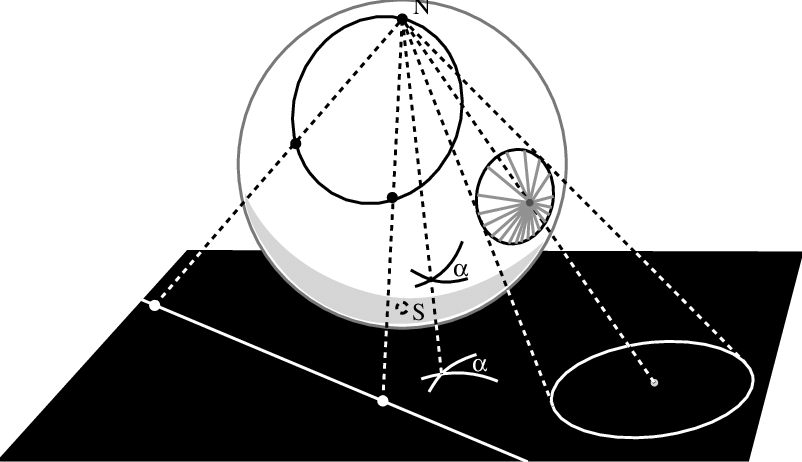
\includegraphics[width=0.28\textwidth]{Stereographic-projection.png}
        }
    }
    \vspace{-3cm}
    \item If $g:U\to\mathbb{C}$, then $Log_\phi(g(z))$ is holomorphic on $g^{-1}(D_{\phi})\cap U$
    \item $Log(z)$ \textit{not continuous} on $\mathbb{C}$. \quad \quad $Log(z)$ not continuous on $Re(z)\leq 0,Im(z)=0$. \\
    \textbf{Remark}: $\log(x)+\log(x)\ne 2\log(x)$
\end{enumerate}

\textbf{Branch Cut|Cut Plane}: \textit{Branch Cut} $L_{z_0,\phi}:=\{z\in\mathbb{C}:z=z_0+re^{i\phi},r\geq0\}$

$\cdot$ \textit{Cut Plane}: $D_{z_0,\phi}:=\mathbb{C}\setminus L_{z_0,\phi}$ \quad {\footnotesize $L_{\phi}=L_{0,\phi};D_{\phi}=D_{0,\phi}$}

$\cdot$ If $Log_{\phi}(z)$ is holomorphic on $D_{\phi}$, then $Log_{\phi}(z-a)$ is holomorphic on $D_{a,\phi}$

\textbf{Branch of Argument}: $Arg_{\phi}(z):=z${\small 的辐角,但是角度限制在:} $\phi<Arg_\phi(z)\leq \phi+2\pi$. \quad \quad ps: {\footnotesize $Arg_{-\pi}(z)=Arg(z)$}

\vspace{-10pt}
\begin{longtable}{cc|cc|cc|cc|cc|cc|cc}
    $f(z)$ & $f'(z)$ & $f(z)$ & $f'(z)$ & $f(z)$ & $f'(z)$ & $f(z)$ & $f'(z)$ & $f(z)$ & $f'(z)$ & $f(z)$ & $f'(z)$ & $f(z)$ & $f'(z)$ \\
    \hline
    $z^n$ & $nz^{n-1}$ & $\exp(z)$ & $\exp(z)$ & $\sin(z)$ & $\cos(z)$ & $\cos(z)$ & $-\sin(z)$ & $\sinh(z)$ & $\cosh(z)$ & $\cosh(z)$ & $\sinh(z)$ & $Log_\phi z$ & $\frac{1}{z}$ {\tiny $z\in D_{\phi}$} \\
\end{longtable}
\vspace{-10pt}

\textbf{Complex Powers}: $z^{\alpha}:=\{\exp(\alpha w):w\in\log(z)\}=\{\exp[\alpha(\ln|z|+iArg(z)+i2k\pi)]:k\in\mathbb{Z}\}$ \quad \qquad \qquad \qquad $\frac{d}{dz}z^\alpha=\alpha z^{\alpha-1}$ {\tiny $z\in D_{\phi}$}

\qquad\textbf{I}. If $\alpha\in\mathbb{Z}$, there is one value of $z^{\alpha}$ \quad \quad \textbf{II}. If $\alpha=\frac{p}{q},\gcd(p,q)=1,p,q\in\mathbb{Z},q\ne0$, there are exactly $q$ values of $z^{\alpha}$

\qquad\textbf{III}. If $\alpha$ is \textit{irrational} or \textit{non-real}, there are infinitely values $z^{\alpha}$ \quad \quad \textbf{IV}. $1^{1/q},q\in\mathbb{Z},q\ne0$ is $\{1,w,...,w^{q-1}\},w=\exp(i2\pi/q)$

\qquad\textbf{V}. We prefer use $\exp(z)$ to denote single-valued function, and $e^z$ to denote multi-valued function. 

\qquad\textbf{Principal Branch}: $z^{\alpha}:=\exp(\alpha Log(z))$ \qquad \qquad \textbf{Operation}: $z^{\alpha}z^{\beta}=z^{\alpha+\beta}$ {\footnotesize (Using Principal Branch)} \quad {\scriptsize \textbf{NB}: $(z_1z_2)^\alpha\ne z_1^\alpha z_2^\alpha \ ; \ (z^\alpha)^\beta\ne z^{\alpha\beta}$}


\section{Conformal Maps and Mobius Transformations} % Conformal Maps and Mobius Transformations

\subsection{Conformal Maps \& Definition of Mobius Transformations} % Conformal Maps & Definition of Mobius Transformations

\textbf{Conformal}: Let $U$ be open set and $f:U\to\mathbb{C}$. Then $f$ is conformal iff: \ \ $f$ \textit{preserves angles}. \quad {\scriptsize i.e.任意两条曲线/直线之间的角度在$f$作用下不变.}

\quad \textbf{Important Theorem}: If $f:U\to\mathbb{C}$ is \textit{holomorphic}, then $\forall z_0\in U,f'(z_0)\ne0$, $f$ \textit{preserves angles}.

\quad i.e. $\forall \ \text{curves} \ C_1,C_2$ in $U$. If $C_1,C_2$ intersecting at a point $z_0\in U$. {\scriptsize $C_1,C_2$在$z_0$切线的夹角与$f(C_1),f(C_2)$在$f(z_0)$切线的夹角一样.}

\textbf{Extended Complex Plane}: $\widetilde{\mathbb{C}}:=\mathbb{C}\cup\{\infty\}$ and define that $a+\infty=\infty,b\cdot\infty=\infty,\frac{b}{0}=\infty,\frac{b}{\infty}=0$.

\textbf{Riemann Sphere}: Consider $(X,Y,Z)\in\mathbb{R}^3$: \ \ $^1z=X+iY\in\mathbb{C}$ is the point $(X,Y,0)$ and \ \ $^2 Z=0$ is the complex plane.

\begin{enumerate}[itemsep=-2pt, topsep=-2pt]
    \item Define the Riemman Sphere: $S^2:=\{(X,Y,Z)\in\mathbb{R}^3:X^2+Y^2+Z^2=1\}$ and consider the \textbf{North Pole} is point $N:=(0,0,1)$
    \item Define $\phi:\mathbb{C}\to S^2$ by \ \ $N$点 与 $z=(X,Y,0)$点 连线 与 $S^2$ 的交点为$\phi(z)$ \quad \quad Thus $\lim_{|z|\to\infty}\phi(z)=N$ \quad $\phi(\infty):=N$
    \item Calculation shows that: $\phi(z)=\phi(x+iy)=\left(\frac{2x}{|z|^2+1},\frac{2y}{|z|^2+1},\frac{|z|^2-1}{|z|^2+1}\right)$ \qquad \qquad $\psi(X,Y,Z)=\begin{cases}\frac{X+iY}{1-Z} , (X,Y,Z)\ne N \\ \infty \quad \ , \ (X,Y,Z)=N\end{cases}$ \\
    \textbf{Remark}: $\phi:\widetilde{\mathbb{C}}\to S^2$ is bijection and it's inverse $\psi:S^2\to\widetilde{\mathbb{C}}$ is the \textbf{stereographic projection}
    \item Stereographic projection $\psi(X,Y,Z)$ maps a circle to either a circle or a straight line. (见上图)
\end{enumerate}

\textbf{Mobius Transformation}: A Mobius Transformation is a function form: $f(z)=\frac{az+b}{cz+d}$ where $a,b,c,d\in\mathbb{C} \ ; \ ad\ne bc$

\begin{enumerate}[itemsep=-2pt, topsep=-2pt]
    \item \textbf{Remark}: $g(z)=\frac{f(z)}{\sqrt{ad-bc}}$ satisfies $ad-bc=1$ \quad $\big|$ \quad If $a,b,c,d$ defined a mobius transformation, then $\lambda a,\lambda b,\lambda c,\lambda d$ also.
    \item For Complex Matrix: $M=\begin{pmatrix}a & b \\ c & d\end{pmatrix}$ with $\det(M) = ad-bc=1$. \quad We define $f_{M}=\frac{az+b}{cz+d}$ \qquad $\begin{matrix}\textbf{I}. f_{M_1M_2}=f_{M_1}f_{M_2} \\ \textbf{II}. f_{M^{-1}}=f_M^{-1} \qquad \end{matrix}$
    \item Extended $f(z)$ from $\mathbb{C}$ to $\widetilde{\mathbb{C}}$ by: $f(-\frac{d}{c})=\infty$ and $f(\infty)=\frac{a}{c}$
    \item {\footnotesize \textbf{Translation}: $f(z)=z+b\Leftrightarrow \begin{pmatrix}1 & b \\ 0 & 1\end{pmatrix}$ \quad \textbf{Rotation}: $f(z)=az,a=e^{i\theta} \ (|a|=1)\Leftrightarrow \begin{pmatrix}e^{i\theta/2} & 0 \\ 0 & -e^{i\theta/2}\end{pmatrix}$ \quad \textbf{Dilation}: $f(z)=rz,r>0 \Leftrightarrow \begin{pmatrix}\sqrt{r} & 0 \\ 0 & 1/\sqrt{r}\end{pmatrix}$} \\
    {\footnotesize \textbf{Inversion}: $f(z)=1/z \Leftrightarrow \begin{pmatrix}0 & i \\ i & 0\end{pmatrix}$ \quad \textbf{$f$ fixes the point at infinity}: If $f(\infty)=\infty$ \ \ {\scriptsize ps: 除了inversion其他都是fix the point at infinity.}}
    \item {\footnotesize \textbf{Theorem}: $f(z)=\frac{az+b}{cz+d}$ be a Mobius Transformation. \ $\Rightarrow$ \ $^1$If $f(\infty)=\infty$: $f$ is a composition of \underline{finite} \textit{Translation, Rotation, Dilation} $\Rightarrow$ $c=0,f(z)=\frac{a}{d}z+\frac{b}{d}$}
    \quad {\footnotesize $^2$ If $f(\infty)<\infty$: $f$ is composition of \underline{finite} \textit{Translation, Rotation, Dilation} and \underline{only one} \textit{inversion}. $\Rightarrow$ $f(z)=\frac{(bc-ad)/c^2}{z+d/c}+\frac{a}{c}$}
\end{enumerate}

\textbf{Properties of Mobius Transformation}: \textit{Important}: $\star$ Möbius transformations map circlines to circlines. $\star$
\begin{enumerate}[itemsep=-2pt, topsep=-2pt]
    \item For mobius transformation $f(z)=\frac{az+b}{cz+d}$, if: \ $\exists z_1,z_2,z_3\in\mathbb{C}$ distinct points. $f(z_1)=z_1,f(z_2)=z_2,f(z_3)=z_3$ $\Rightarrow$ $f$ is identity.
    \item If $z_1,z_2,z_3\in\widetilde{\mathbb{C}}$ distinct points. \quad $\exists!$ mobius transformation $f(z)$ s.t. $f(z_1)=1,f(z_2)=0,f(z_3)=\infty$
    \item If $(z_1,z_2,z_3),(w_1,w_2,w_3)\in\widetilde{\mathbb{C}}$ distinct points. Then $\exists!$ mobius transformation $f(z)$ s.t. $f(z_i)=w_i \ , \ \forall i\in\{1,2,3\}$ \\
    \textbf{ps:Method to construct $2$}: If $z_i<\infty,f(z)=\frac{z_1-z_3}{z_1-z_2}\cdot\frac{z-z_2}{z-z_3}$ \qquad If $z_i=\infty$, {\footnotesize $f(z)=\frac{z-z_2}{z-z_3}$ {\scriptsize ,$z_1=\infty$} $f(z)=\frac{z_1-z_3}{z-z_3}$ {\scriptsize ,$z_2=\infty$} ; $f(z)=\frac{z-z_2}{z_1-z_2}$ {\scriptsize ,$z_3=\infty$} } \\
    \textbf{ps:Method to construct $3$}: For 3: Let $f:=h^{-1}\circ g$ {\footnotesize where $g(z_i),h(w_i)=\{1,0,\infty\}$ like part 2.}
    \vspace{1.5pt}
\end{enumerate}

\textbf{Cross-Ratio}: cross-ratio $[z_1,z_2,z_3,z_4]:=f(z_1)$ where $f$ is mobius transformation s.t. $f(z_2)=1,f(z_3)=0,f(z_4)=\infty$

\begin{enumerate}[itemsep=-2pt, topsep=-2pt]
    \item \textbf{Formulas}: {\footnotesize $[z_1,z_2,z_3,z_4]=\frac{z_1-z_3}{z_1-z_4}\frac{z_2-z_4}{z_2-z_3}$ \quad $[\infty,z_2,z_3,z_4]=\frac{z_2-z_4}{z_2-z_3}$ \quad $[z_1,\infty,z_3,z_4]=\frac{z_1-z_3}{z_1-z_4}$ \quad $[z_1,z_2,\infty,z_4]=\frac{z_2-z_4}{z_1-z_4} \quad [z_1,z_2,z_3,\infty]=\frac{z_1-z_3}{z_2-z_3}$}
    \item \textbf{Theorem}: If $f$ is a mobius transformation, $[f(z_1),f(z_2),f(z_3),f(z_4)]=[z_1,z_2,z_3,z_4]$ \qquad \quad {\scriptsize \textbf{$z_i$'s in this "small section" are distinct.}}
\end{enumerate}

\end{document}